\chapter{CPU部分}

\section{流水线结构}
\subsection{基本单发射结构}
流水线可以将一条指令的指令拆分成多个较小的步骤,每个步骤都可以按照更高的频率运行从而能够提高CPU的最终运行频率。通常可以将指令的执行划分成为5级流水线
\begin{itemize}
	\item \textbf{取指(IF)}:从内存中读取需要执行的指令。
	\item \textbf{译码(ID)}:将指令进行译码。同时读取指令所需要寄存器值,解析指令码中的立即数并进行扩展,对跳转指令给出跳转地址。
	\item \textbf{执行(EX)}:按照译码阶段的指令类型,给出对应结果。
	\item \textbf{访存(MM)}:如果需要访问内存,则在这一阶段进行。
	\item \textbf{回写(WB)}:将运算结果保存到对应寄存器。
\end{itemize}

\begin{figure}[htbp]
	\centering
	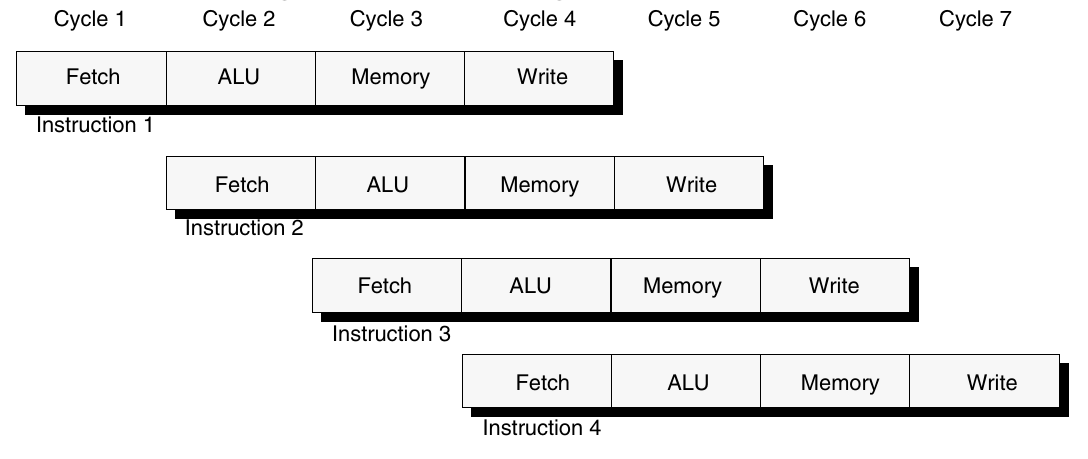
\includegraphics[width=\linewidth]{standard-pipeline.png}
	\caption{标准的流水线结构,图示中没有绘制出译码阶段。}
	\label{fig:standard-pipeline}
\end{figure}

流水线结构本身在带来性能的提升的同时还会带来一部分冒险问题,有以下三种
\begin{itemize}
	\item \textbf{结构冒险}:多条指令对同一资源进行访问。例如访存和取指同时对一个地址进行访问。
	\item \textbf{数据冒险}:流水线内部一条指令依赖于上一条指令的执行结果。
	\item \textbf{控制冒险}:在ID阶段才能确定跳转地址,但IF阶段就需要获取指令。
\end{itemize}

在MIPS架构中,如果按照如上五级流水线结构实现,则不会出现控制冒险。因为对于跳转指令,其下一条指令无论跳转与否均会执行,这样IF阶段获取的指令刚好能够继续指令。

对于数据冒险有两个方法进行解决:

\begin{itemize}
	\item \textbf{数据旁路}:将计算结果直接送到需要的地方。比如将EX阶段的结果直接送到ID阶段。
	\item \textbf{流水线暂停}:插入空指令,暂停流水线的运行。
\end{itemize}

\subsection{双发射流水线的设计}
双发射是指在一个时钟周期内可以执行两条的CPU指令,更一般地,在一个周期同时内执行多条CPU指令的技术叫做超标量技术,其流水线结构如图\ref{fig:superscalar}所示。双发射能够有效地提高CPU的效率,但是它同时也对流水线的设计带来了一定程度的挑战。

\begin{figure}[htbp]
	\centering
	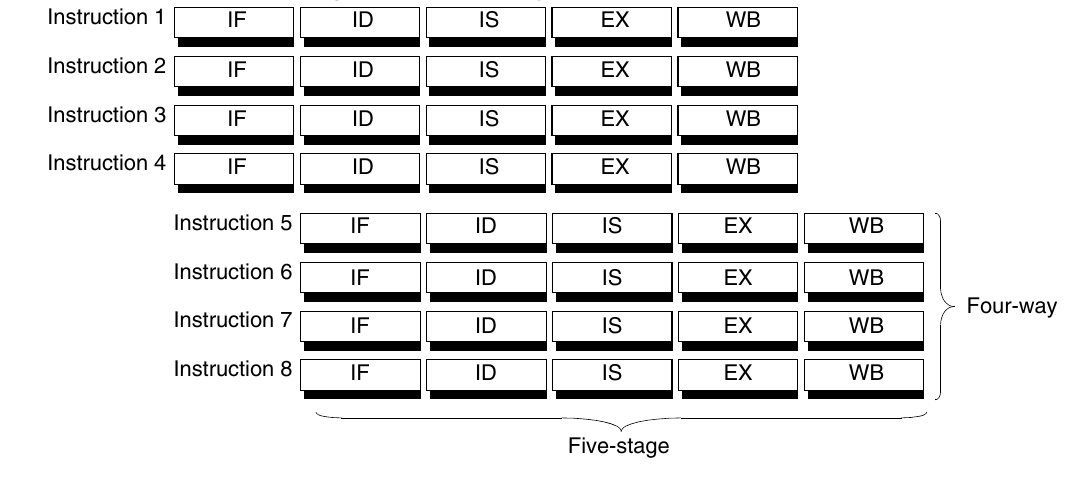
\includegraphics[width=\linewidth]{superscalar.png}
	\caption{超标量流水线结构。}
	\label{fig:superscalar}
\end{figure}

在我们的设计中,对于大部分的指令组合来说流水线是可以两条同时执行的。其结构的设计与标准单发射流水线的主要不同在于IF和ID阶段对指令发射的控制,具体来说有这样两点
\begin{enumerate}
	\item 在IF阶段对PC的修改要保证接下来一个阶段有两条新的指令。因为在取指完成后无法判断这两条指令是否能够一起发射,因此对PC的修改要考虑的是最好情况,也就是它们能够一起发射,但是到了ID阶段,如果这两条指令没有一起发射,那么PC就相当于超前了,这时候就需要针对各个情况进行不同处理。
	\item 在ID阶段译码完成后,需要决定当前的两条指令是否可以同时发射。需要判断的情况较多,例如两条算术指令是否有数据相关,是否是SSNOP这样的特殊指令,是否是分支指令等。
\end{enumerate}

根据ID阶段对何种指令可以同时发射的控制,之后EX和MEM阶段的处理也会有不同之处。这部分内容在我们叙述完这两个部分之后再进行讨论。

在此之前,我们假设从总线获取的指令数据宽度是64位,也就是一次给出一个物理地址,获取64位的数据。

\subsubsection{指令发射控制}
如上所述,在译码阶段需要控制指令是否能够同时发射。如果可以同时发射,那么就把两条指令送给下一阶段,如果判定第二条指令不能够发射,则将其设置为NOP,并且保持第一条不动送给下一阶段。之后执行阶段就可以无需考虑当前两条指令是否是同时发射。

下面是我们实现中\textbf{不能}够同时发射的指令组合,我们称同时发射的两条指令分别为A和B

\begin{itemize}
\item \textbf{Superscalar No Operation} 这是一条类似NOP的指令,其指令代码是SSNOP。在MIPS规范中该条指令必须单独占用一个时钟周期,不能够和其它指令一起发射。

\item \textbf{条件移动指令的数据相关}\ 若指令B为条件移动指令,并且A和B有数据相关,即指令B需要读取指令A需要写的寄存器。由于我们在ID阶段决定寄存器的写信号,需要寄存器的值,而指令B需要的寄存器值在EX阶段才能够获取,因此不同时发射。

\item \textbf{多周期指令的数据相关}\ 对于多周期指令(例如MADDU和FPU指令)如果指令A和B有数据相关,那么不能同时发射。注意对于单周期指令,无论是否有数据相关,我们都可以同时发射。

\item \textbf{分支、特权指令}\ 出于实现方便,指令B不能为分支或者CP0指令。

\item \textbf{延迟槽指令}\ 若指令A为延迟槽,那么下一条指令不能与其一起发射。

\item \textbf{内存相关指令}\ 由于数据总线仅一条,我们只支持A和B中最多有一条访存指令。

\item \textbf{TLB边界指令}\ 如果虚拟地址在TLB边界,其对应的物理地址可能是不连续的,因此此类指令不能够同时发射。因为获取的第二条指令可能无效。这一条是较为特殊的,对之后指令获取的预测部分有较大的影响。
\end{itemize}

\subsubsection{指令获取预测}
指令获取的预测较为复杂,影响该部分的因素主要有二:总线送来的两条物理地址连续的指令是否在虚拟地址上是连续的;上一个周期的两条指令是否同时发射。

预测的原则是需要寻找一个方法,保证在IF阶段对PC的增量进行决策,使得无论当前两条指令是否在ID阶段同时发射,在下一个周期读取得到的两条指令都能够保证双发射的需求。这部分的实现主要是一个有3个不同状态的状态机。

\begin{figure}[htbp]
	\centering
	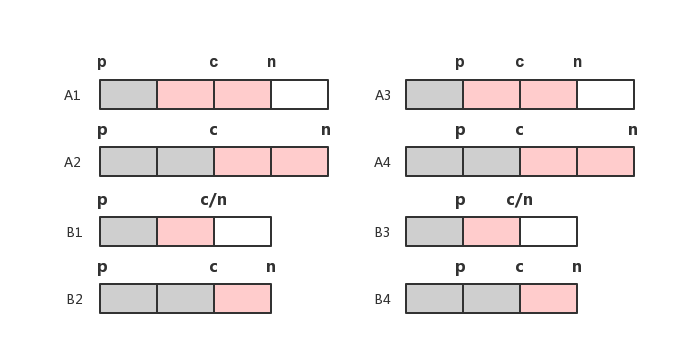
\includegraphics[width=4.3in]{emit-prediction.png}
	\caption{指令获取预测中可能出现的8种情况。灰色部分表示ID发射的指令,红色部分表示IF阶段读取的指令,p表示上一周期PC的位置,c表示当前PC位置,n表示下一周期PC应该在的位置。}
	\label{fig:emit-prediction}
\end{figure}

该状态机的状态的意义及其对应的转移如下,在每次转移我们可以得到的信息是ID阶段两条指令是否同时发射,以及它们是否在虚拟地址上是连续的(对应跨TLB边界的情况)。对应于当前PC,上一周期的PC和下一周期应该设置的PC值的8种可能如图\ref{fig:emit-prediction}。
\begin{itemize}
	\item \texttt{HARD\_SET} 这表示PC是刚刚经过初始化,或者通过一条转移指令或异常刷新设置而来的,而不是通过PC自身自增得到。
	\item \texttt{MATCH}
	\item \texttt{AHEAD}
\end{itemize}<++>

\subsubsection{指令的执行和``数据下推''}
在不考虑数据相关的情况下,指令的执行只需要简单地生成出两个相同的ALU即可。由于我们的设计中,有数据相关的单周期指令也可以同时发射,这样需要进行额外的处理来解决这个相关问题。我们解决的方法类似于``数据前推'',具体的实现是将指令A的ALU计算结果直接通过组合逻辑送到指令B的ALU,再根据情况进行选择。这种实现我们称为``数据下推''。

另外,在访存阶段,由于双发射控制中已经排除了两条指令同时访存的情况,这阶段只需要判断两条指令是否有其一访存再进行对应的处理即可。

\begin{landscape}
\begin{figure}[htbp]
	\centering
	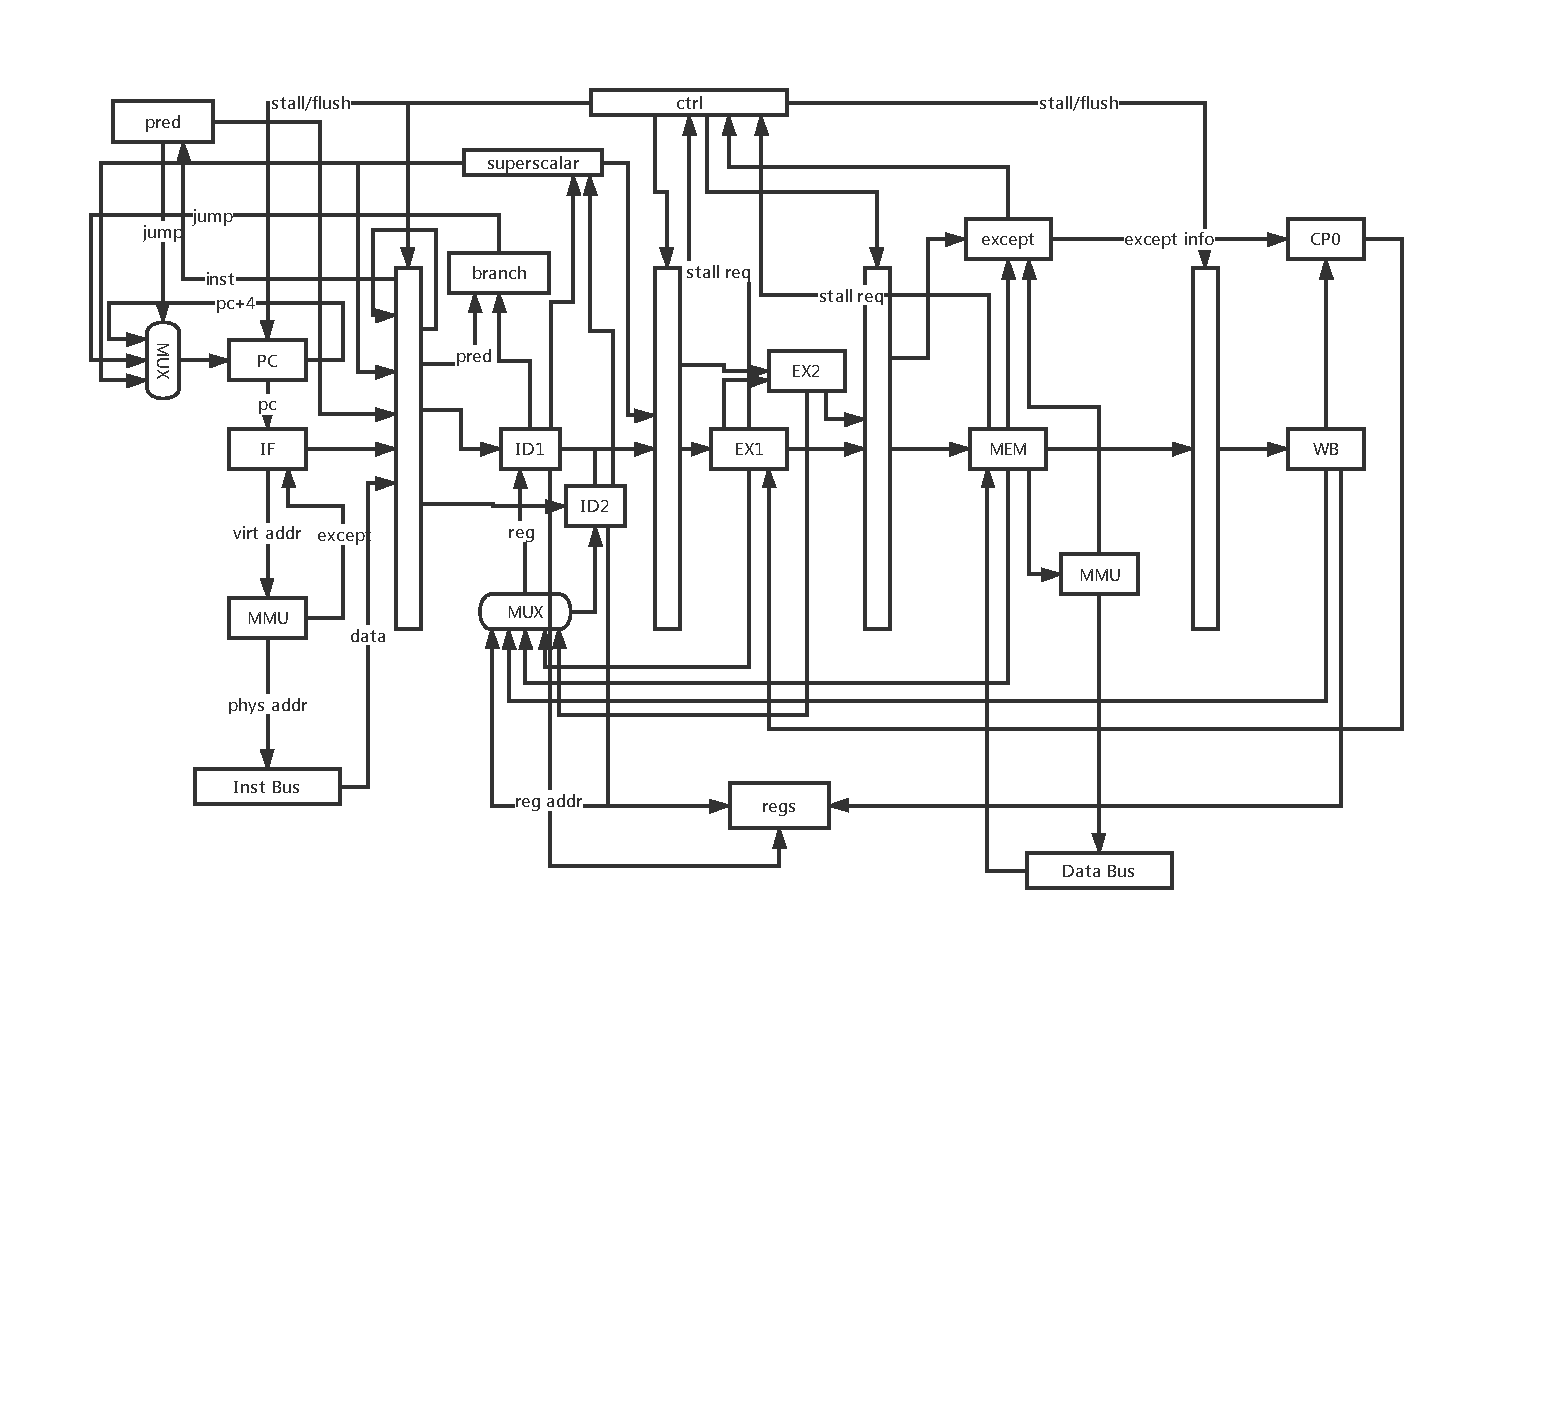
\includegraphics[width=\linewidth]{datapath.pdf}
	\caption{CPU数据通路,仅绘制出大致的结构,具体的信号见文字描述。}
	\label{fig:cpu-datapath}
\end{figure}
\end{landscape}
\section{指令集}
下方按照功能划分列举了CPU所支持的MIPS指令,各条指令的具体编码以及功能在MIPS文档中有详细的描述。
\begin{itemize}
	\item \textbf{自陷指令} TGE, TEGU, TLT, TLTU, TEQ, TNE, TGEI, TGEIU, TLTI, TLTIU, TEQI, TNEI
	\item \textbf{分支指令} BLTZ, BGEZ, BLTZAL, BGEZAL, BEQ, BNE, BLEZ, BGTZ, JR, JALR, J, JAL
	\item \textbf{逻辑指令} AND, OR, XOR, ANDI, ORI, XORI, NOR, SLL, SRL, SRA, SLLV, SRLV, SRAV
	\item \textbf{算术指令} ADD, ADDU, SUB, SUBU, ADDI, ADDIU, MUL, MULT, MULTU, DIV, DIVU, MADD, MADDU, MSUB, MSUBU, CLO, CLZ
	\item \textbf{访存指令} SB, SH, SW, SWL, SWR, LB, LH, LWL, LWR, LW, LBU, LHU, LL, SC
	\item \textbf{特权指令} SYSCALL, BREAK, TLBR, TLBWI, TLBWR, TLBP, ERET, MTC0, MFC0
	\item \textbf{条件移动指令} SLT, SLTU, SLTI, SLTIU, MOVN, MOVZ
	\item \textbf{无条件移动指令} LUI, SLT, SLTU, MFHI, MFLO, MTHI, MTLO 
\end{itemize}

\section{协处理器0}
CP0是MIPS规范中必要的一个协处理器,它提供了操作系统所必须的功能抽象,例如异常处理、内存管理和资源访问控制等。

在CP0中有多个32位寄存器,各个寄存器均通过MTC0和MFC0读写。另外,诸如TLBWI、TLBWR和TLBP等特权指令还有异常的发生也有可能会影响其值。

表\ref{table:required_cp0_registers}中列出了必须实现的CP0寄存器。

\begin{table}[!htbp]
    \centering
    \begin{tabular}{|r|l|l|}
    \hline
    \textbf{编号} & \textbf{名称} & \textbf{功能}  \\ \hline
	8 & BadVAddr & 最近发生的与地址相关的异常所对应的地址 \\ \hline
	9 & Count & 计数器 \\ \hline
	11 & Compare & 计时中断控制器 \\ \hline
	12 & Status & 处理器状态及控制 \\ \hline
	13 & Cause & 上一次异常的原因 \\ \hline
	14 & EPC & 上一次异常发生的地址 \\ \hline
	15 & PEId & 处理器版本和标识符 \\ \hline
	16 & Config & 处理器配置 \\ \hline
	30 & ErrorEPC & 上一次异常发生的地址 \\ \hline
    \end{tabular}
    \caption{必要的CP0寄存器}
    \label{table:required_cp0_registers}
\end{table}

为了实现TLB MMU的功能,还需要表\ref{table:mmu_cp0_registers}中所列出的寄存器。

\begin{table}[!htbp]
    \centering
    \begin{tabular}{|r|l|l|}
    \hline
    \textbf{编号} & \textbf{名称} & \textbf{功能}  \\ \hline
	0 & Index & TLB数组的索引 \\ \hline
	1 & Random & 随机数 \\ \hline
	2 & EntryLo0 & TLB项的低位 \\ \hline
	3 & EntryLo1 & TLB项的低位 \\ \hline
	4 & Context & 指向内存中页表入口的指针 \\ \hline
	5 & PageMask & 控制TLB的虚拟页大小 \\ \hline
	6 & Wired & 控制TLB中固定的页数 \\ \hline
	10 & EntryHi & TLB项的高位 \\ \hline
    \end{tabular}
    \caption{MMU所需要的CP0寄存器}
    \label{table:mmu_cp0_registers}
\end{table}

同时,为了支持自定义异常向量,还需要额外实现一个MIPS 32 Rev 2 中的 EBase寄存器。

\section{中断和异常}
\subsection{中断}
MIPS的中断一共有8个,从0开始编号。其中0号中断和1号中断是软件中断,由软件设置Cause寄存器中的对应位来触发。其余6个中断为硬件中断,由外部硬件触发。在实现中,由Count/Compare寄存器组合而成的定时中断的中断号为7。

\subsection{异常}
MIPS的异常是“精确异常”,也就是在异常发生前的指令都会执行完毕,异常发生之后的指令不会继续执行。在异常发生时,CPU会跳转到对应的异常向量处执行异常处理代码并设置CP0中对应的寄存器记录异常的原因和一些额外的信息,同时还会进入Kernel Mode。处理异常代码的异常向量由“基地址+偏移”来决定,偏移是根据异常来确定的,基地址是由CP0的EBase寄存器决定。

需要支持的异常在表\ref{table:main-exception}中列出。

\begin{table}[htbp]
	\centering
	\begin{tabular}{|c|c|l|} \hline
		\textbf{异常简称} & \textbf{异常说明} \\ \hline
		Int & 中断  \\ \hline
		Mod & TLB修改异常 \\ \hline
		TLBL & TLB Load异常 \\ \hline
		TLBS & TLB Store异常 \\ \hline
		AdEL & 地址Load异常 \\ \hline
		AdES & 地址Store异常 \\ \hline
		Sys & 系统调用 \\ \hline
		Bp & 断点 \\ \hline
		RI & 保留指令 \\ \hline
		CpU & 协处理器不可用 \\ \hline
		Ov & 算术溢出 \\ \hline
		Tr & 自陷异常 \\ \hline
	\end{tabular}
	\caption{主要支持的异常}
	\label{table:main-exception}
\end{table}
\section{内存管理}
MIPS为操作系统的内存管理提供了较为简单的支持,虚拟地址通过MMU转换为物理地址。MIPS标准对虚拟地址和物理地址的映射如表\ref{tab:virtual-address-space}所示。

\begin{table}[htbp]
	\centering
	\begin{tabular}{|c|c|c|c|} \hline
		\textbf{段} & \textbf{虚拟地址} & \textbf{权限} & \textbf{物理地址} \\ \hline
		kseg3/ksseg & \texttt{0xC000000-0xFFFFFFFF} & Kernel & 由TLB转换 \\ \hline
		kseg1 & \texttt{0xA0000000-0xBFFFFFFF} & Kernel & \texttt{0x00000000-0x1FFFFFFF} \\ \hline
		kseg0 & \texttt{0x80000000-0x9FFFFFFF} & Kernel & \texttt{0x00000000-0x1FFFFFFF} \\ \hline
		useg &  \texttt{0x00000000-0x7FFFFFFF} & User & 由TLB转换 \\ \hline
	\end{tabular}
	\caption{虚拟地址空间}
	\label{tab:virtual-address-space}
\end{table}

具体的地址转换由TLB来完成,TLB可以认为是在CPU内部的地址转换表的高速缓存。具体的内容需要由操作系统来进行填充。如果在TLB中没有找到对应虚拟地址则会触发一个TLB miss异常,操作系统对该异常处理,并且将对应转换表填入TLB中的某一项来完成对地址的转换。
